% !TeX encoding = ISO-8859-1
\chapter{Anwendungen von Algorithmen}
%Grundeinleitung
%Nachdem die Grundlagen der Funktionsprinzipien der Algorithmen zu Pfadplanung nun erl�utert  wurden, wird nun auf m�gliche Anwendungen dieser eingegangen.
\section{Anwendungen mit diskretem Zustandsraum}
Die Klassifizierung des Planens im  diskreten Zustandsraum ist z.B. f�r das Rubik's Cube R�tsel zutreffend (siehe Abb. \ref{Abb. 5.1}), bei dem es ebenso einen endlichen Zustandsraum und einen endlichen Aktionsrahmen gibt. Der Zustandsraum ist hierbei die Summe aller Zust�nde, die der W�rfel annehmen kann, also jegliche m�gliche Farbverteilung. Der Aktionsrahmen ist die Menge aller Richtungen, in die man jedes Element drehen kann. Der bestm�gliche Pfad ist in diesem Fall die geringste Anzahl an Drehungen des W�rfels in der richtigen Reihenfolge, um ans Ziel bzw. zum Zielzustand zu gelangen, welcher ist, dass jede Seite des W�rfels nur noch Elemente einer Farbe hat.\cite[~S. 20]{Lav06}\\
\begin{figure}
	\centering
	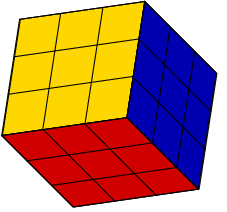
\includegraphics[width=0.4\linewidth]{images/img229}
	\caption{in Anlehnung Abb. 1.1 von \cite[~S. 5]{Lav06}: Rubik's Cube.}
	\label{Abb. 5.1}
\end{figure}

Die n�chste Anwendung ist die Bewegungen eines Roboters oder einer K�nstlichen Intelligenz auf einem 2D Netz. Dies geschieht in Strategie-Computerspielen, in denen eine Figur von ihrem aktuellen Standpunkt zu einem Ort gelangen muss, der ihr zugewiesen wird. Hier kommt der Pfadplanungsalgorithmus zum Einsatz.\cite{cui2011based}%genauer drauf neue Quelle eingehen.\\
%s27ff
\section{Anwendungen zur Planung mit kontinuierlichem Zustandsraum}
Wie in Kapitel \ref{Kapitel 4.2} schon erw�hnt, klassifiziert man bei den Algorithmen zur Planung mit kontinuierlichem Zustandsraum zwischen drei verschiedenen Rubriken, die unterschiedliche Anwendungsbereiche haben, auf die im Folgenden einzeln eingegangen wird.
\subsection{Anwendungen zur Planung mit allen Umgebungsinformationen vorhanden}
Ein gutes Beispiel f�r Anwendungen zur Planung, bei der alle Umgebungsinformationen vorhanden sind, ist das bereits in \ref{Kapitel 4.2} angesprochene Piano Mover's Problem.\\
Eine praktische Anwendung ist das digitale Planen von Fabrik-Robotern, die ein Auto zusammensetzen sollen. In Abb. \ref{Abb. 5.2} ist das digitale Planen des automatischen An- und Abmontierens eines Scheibenwischermotors an ein Auto mittels eines CAD Modells dargestellt.
\begin{figure}
	\centering
	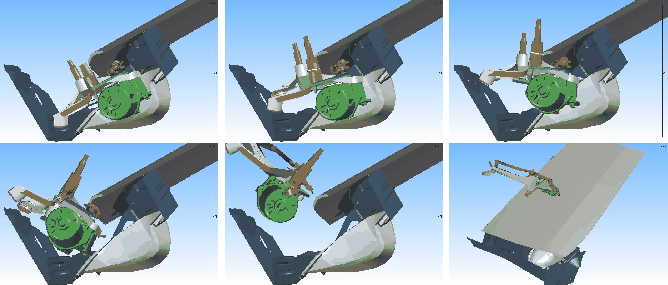
\includegraphics[width=0.7\linewidth]{images/img231}
	\caption{Abb. 1.3 von \cite[~S. 7]{Lav06}: Eine Auto-Montierungsaufgabe, die beinhaltet, dass ein Scheibenwischermotor an ein Auto angebracht oder entfernt werden soll.}
	\label{Abb. 5.2}
\end{figure}

Eine Software muss entscheiden, ob und wie der Scheibenwischermotor an- und abmontiert werden kann, oder nicht. Das fr�her zeit- und kostenintensive Entwickeln des Designs wird nun mit Software vereinfacht, indem CAD Modelle manipuliert werden. Auch hier hat man einen �berabz�hlbar unendlichen Zustandsraum und alle Umgebungsinformationen sind bekannt. \cite[~S. 6 ff]{Lav06}
%part 2 QUELLE ANGEBEN
\subsection{Anwendungen zur Planung mit Unsicherheit}
Bei der Planung mit Unsicherheit (engl. planning under uncertanty), auch \textit{decision-theoretic planning} genannt, interferieren Ungewissheiten im Allgemeinen mit 2 Aspekten des Planens. Diese beiden Aspekte sind Vorhersehbarkeit und Wahrnehmung. \cite[~S. 435 ff.]{Lav06}\\
Die Vorhersehbarkeit ist in dem Sinne durch die Unsicherheiten beeintr�chtigt, dass nicht bekannt ist, was passieren wird, wenn gewisse Aktionen ausgef�hrt werden. Die Wahrnehmung ist durch die Unsicherheiten beeintr�chtigt, da der aktuelle Status, bzw. die aktuelle Position nicht bekannt ist. Denn den Status erh�lt man aus den Ausgangsbedingungen, den Sensoren und den Informationen �ber die vorangegangenen Aktionen.\\
Ein Beispiel f�r eine solche Anwendung ist das Autonome Fahren im Allgemeinen. %Quellen suchen
 Hier bewegt sich das Auto nicht �ber ein festes 2D Netz, sondern durch die unvorhersehbare Realit�t. Der Bordcomputer des Autos nimmt durch seine Sensoren und eventuelle Au�enkameras seine Umgebung wahr und versucht durch diese und GPS-Daten, seinen Status bzw. seine aktuelle Position herauszufinden. Da sich jedoch die Umgebung stets ver�ndert und das Verhalten der anderen Verkehrsteilnehmer nicht vorhersagbar ist, kommt die Unsicherheit ins Spiel.
Dies l�sst sich auf die Navigation von allen mobilen Robotern �bertragen.
Da der aktuelle Status nie gewiss sein kann, wird mit allen verf�gbaren Informationen versucht, den Status so genau wie m�glich zu bestimmen.
%(s.25) Part 3
\subsection{Anwendungen zur Planung mit Bewegungseinschr�nkungen}
Bei Anwendungen zur Planung mit Bewegungseinschr�nkungen (engl. planning under differential constraints) muss beachtet werden, dass der schnellste Pfad, der errechnet wird, oft durch Bewegungseinschr�nkungen nicht umgesetzt werden kann. In der Robotik entstehen diese Bewegungseinschr�nkungen h�ufig durch die Kinematik und Dynamik der Roboter selbst.\\
Auch hier kann gut das Auto als Beispiel herhalten. Ein Auto kann nicht seitw�rts fahren. Wenn es also seitlich neben einer Parkl�cke steht und man mit Hilfe des Einparkassistenten das Auto einparken lassen will, w�re der k�rzeste Pfad seitw�rts zu fahren. Da dies nicht m�glich ist, muss das bei der Pfadplanung ber�cksichtigt werden (siehe Abb. \ref{Abb. 5.3}).
\begin{figure}
	\centering
	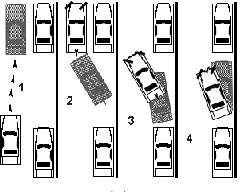
\includegraphics[width=0.5\linewidth]{images/img239}
	\caption{in Anlehnung an Abb. 1.11 von \cite[~S. 15]{Lav06}}
	\label{Abb. 5.3}
\end{figure}

%s26 Part IV